\section{Motivation}

In this section, we motivate the need for a formal reasoning framework
for weakly isolated transactions through a series of examples. All our
examples are written in C-like imperative language equipped with a
\C{txn} lexical block for transactions. Each \C{txn} block is
associated with a single-quoted string in angle braces that uniquely
identifies the transaction. We use Hoare triple notation to annotate
programs with pre and post conditions.

\begin{figure}
\centering
$\{\{\texttt{C}=\texttt{k} \conj \texttt{k}\ge\texttt{a1+a2}\}\}$
\begin{tabular}{l||l}
\begin{txnimpcode}
  txn$\langle$'Wd1'$\rangle${
    if (C $\ge$ a1) {
      C := C - a1
    }
  }
\end{txnimpcode}
&
\begin{txnimpcode}
  txn$\langle$'Wd2'$\rangle${
    if (C $\ge$ a2) {
      C := C - a2
    }
  }
\end{txnimpcode}
\\
\end{tabular}
$\{\{\texttt{C}=\texttt{k-a1-a2}\}\}$

\caption{Concurrent withdraw transactions}
\label{fig:motiv-eg-1}
\end{figure}

Consider an implementation of a banking application that admits
concurrent withdraw transactions on a checking account (\C{C}), as
shown in Fig.~\ref{fig:motiv-eg-1}. If the initial balance (\C{k}) in
the account is enough to perform both withdraws, then the final
balance, after both transactions commit, is expected to reflect the
effects of both withdraws. The pre and post conditions in
Fig.~\ref{fig:motiv-eg-1} reflect our expectations. Indeed, invariants
are guaranteed to hold if both withdraw transactions are serialized,
making \iso{Serializable} isolation (SER) level a sufficent condition
to preserve invaraints. But, is SER necessary?

% Most weak isolation levels allow executions to interleave operations
% (Reads, Writes and Commits) of one transaction with other's, while
% enforcing some additional constraints. Arbitrary interleavings may
% lead to the violation of invaraints. 
Let us consider \iso{Read Committed} (RC), an isolation level weaker
than SER that is default in Postgres 9.5~\cite{postgres95} and Oracle
11g~\cite{oracle11g} databases. An RC transaction is isolated from the
writes of an uncommitted transactions, thus preventing the so called
\emph{dirty reads} phenomenon~\cite{berenson}. In the current example,
RC isolation admits following executions:

\begin{figure}[!h]
\centering
\subcaptionbox {
  RC Execution 1
  \label{fig:motiv-eg-1-a}
} [
  0.55\columnwidth
] {
  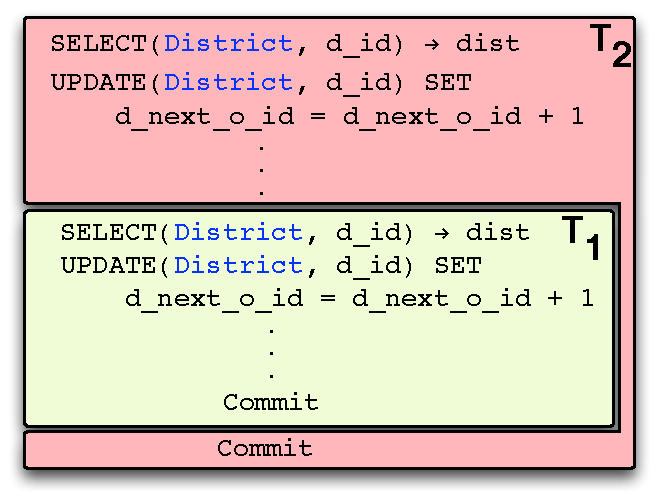
\includegraphics[scale=0.5]{Figures/motiv-eg-1-a}
}
%\hspace*{0.5in}
\subcaptionbox {
  RC Execution 2
  \label{fig:motiv-eg-1-b}
}{
  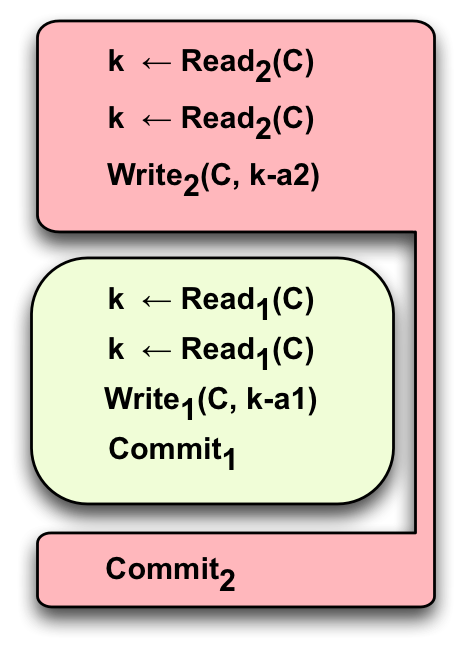
\includegraphics[scale=0.5]{Figures/motiv-eg-1-b}
}
\end{figure}

An execution is a series of Read, Write and Commit operations.
Subscript of an operation indicates its transaction. For clarity,
effects of different transactions are shown against differently
colored backgrounds. In the first execution, the first transaction
(`Wd1') reads the current balance (\C{k}) and writes the new balance
(\C{k-a1}), but before it commits transaction `Wd2' executes and
commits, writing the new balance (\C{k-a2}). RC isolation has
prevented `Wd2' from witnessing the writes of uncommitted transaction
`Wd1'. Committing `Wd1' now leads to the loss of updates from `Wd2'
(the so called \emph{lost update anomaly}~\cite{berenson}), resulting
in a balance of \C{k-a1}. The second execution describes a similar
scenario with `Wd1' and `Wd2' exchanging their roles. 

Clearly, \iso{Read Committed} is not sufficient because it loses the
updates of one transaction and violates the invariant in
Fig.~\ref{fig:motiv-eg-1}. Now, consider an alternative unfolding of
Execution 1, where, rather than committing `Wd1' and overwriting the
updates of `Wd2', we rollback `Wd1' to reexecute it starting from the
state that contains the updates of `Wd2'. No updates are lost in this
alternative execution, leading to the satisfaction of
Fig.~\ref{fig:motiv-eg-1} invariant. Rolling back and reexecuting an
uncommitted transaction to prevent write-write conflicts with a
committed transaction is a strategy often adopted by databases to
implement \iso{Snapshot Isolation} (SI) level. Indeed, SI is
sufficient to enforce the required invaraints in this
example\footnote{\iso{Parallel Snapshot Isolation} (PSI), a weaker
version of SI tailor-made for replicated stores is also sufficient.}.
Moreover, relying on optimistic speculation instead of pessimistic
locking for concurrency control makes SI more efficient than SER,
making it appropriate for transactions in Fig.~\ref{fig:motiv-eg-1}.
Note that we have arrived at his judgment via adhoc reasoning based on
speculations about database's implementation strategies. Such a
reasoning process is necessarily fragile and error-prone. Is there a
better way?

\begin{figure}
\centering
$\{\{\texttt{C+S}\ge\texttt{0}\}\}$
\begin{tabular}{l||l}
\begin{txnimpcode}
  txn$\langle$'WdC'$\rangle${
    if (C+S $\ge$ a1) {
      C := C - a1
    }
  }
\end{txnimpcode}
&
\begin{txnimpcode}
  txn$\langle$'WdS'$\rangle${
    if (C+S $\ge$ a2) {
      S := S - a2
    }
  }
\end{txnimpcode}
\\
\end{tabular}
$\{\{\texttt{C+S}\ge\texttt{0}\}\}$

\caption{Withdraws from current (\C{C}) and savings (\C{S}) accounts.}
\label{fig:motiv-eg-2}
\end{figure}

\iso{Snapshot Isolation} effectively serializes updates to a data
object without necessarily relying on expensive lock-based concurrency
control. While this makes it a better alternative to
\iso{Serializable} isolation, it is however not a replacement for the
latter. Consider a different banking application that maintains a
current (\C{C}) and savings account (\C{S}) for each user. A user can
withdraw either from current or from savings account as long as the
combined balance is at least as much as the amount being withdrawn.
Fig.~\ref{fig:motiv-eg-2} shows a pair of concurrent transactions,
`WdC' and `WdS', performing withdraws from current and savings
accounts, respectively. Pre and post conditions assert non-negative
combined balance invariant. \iso{Serializable} isolation is sufficient
to preserve the invariant, but \iso{Snapshot Isolation} is not.
Intuitively, this is because there are no \emph{lost updates} in this
example even when both transactions commit concurrently, hence there
is no reason for SI to effectively serialize them. A reasoning
framework for weak isolation should let us formally deduce this fact
by making it impossible to construct a proof of correctness for the
program under SI, but facilitating a proof under SER.

\begin{figure}[t]
\centering
$\{\{\texttt{C+S}\ge\texttt{0}\}\}$
\begin{tabular}{l||l||}
\begin{txnimpcode}
  txn$\langle$'Xfer'$\rangle${
    C := C - a;
    S := S + a;
  }
\end{txnimpcode}
&
\begin{txnimpcode}
  txn$\langle$'TotBal'$\rangle${
    T := S + C
  }
\end{txnimpcode}
% \\
% \multicolumn{2}{c} {
% }
\end{tabular}
\begin{tabular}{c}
  \begin{txnimpcode}
    txn$\langle$'AddInt'$\rangle${
      S := S + (T*0.1)
    }
  \end{txnimpcode}
\end{tabular}

$\{\{\texttt{C+S}\ge\texttt{0}\}\}$

\caption{Concurrent transfer (\C{Xf}) and interest accumulation (\C{Int}).}
\label{fig:motiv-eg-3}
\end{figure}

The previous two examples preserve invariants on \C{C} and \C{S} by
effectively serializing transactions that write to \C{C} and \C{S}.
However, in general, serializing a subset of transactions that write
to the data objects referred by invariants is neither sufficient nor
necessary to uphold the invariants. Consider the banking application
in Fig.~\ref{fig:motiv-eg-3} with three transactions. Transaction
`Xfer' transfers some amount (\C{a}) from current (\C{C}) to savings
(\C{S}) account.  Transaction `TotBal' records the total balance in
both the accounts in a data object \C{T}, and transaction `AddIntr'
calculates interest on total balance (10\% of \C{T}) and adds it to
the savings account. Using a data object to record some function of
the current state of other data objects is a standard practice in
relational databases, where Materialized Views~\cite{oraclematview}
are created to maintain the results of a SQL query. Like the previous
example, the invariant of interest in this example is non-negative
total balance; if we start with a non-negative total balance, and we
add interest based on the total balance, we must end up with a
non-negative total balance.  However, unlike the previous example,
serializing transactions that write to \C{C} and \C{S} is not
sufficient to guarantee the invariant.  The following execution
demonstrates this anomaly:

\begin{figure}[!h]
\centering
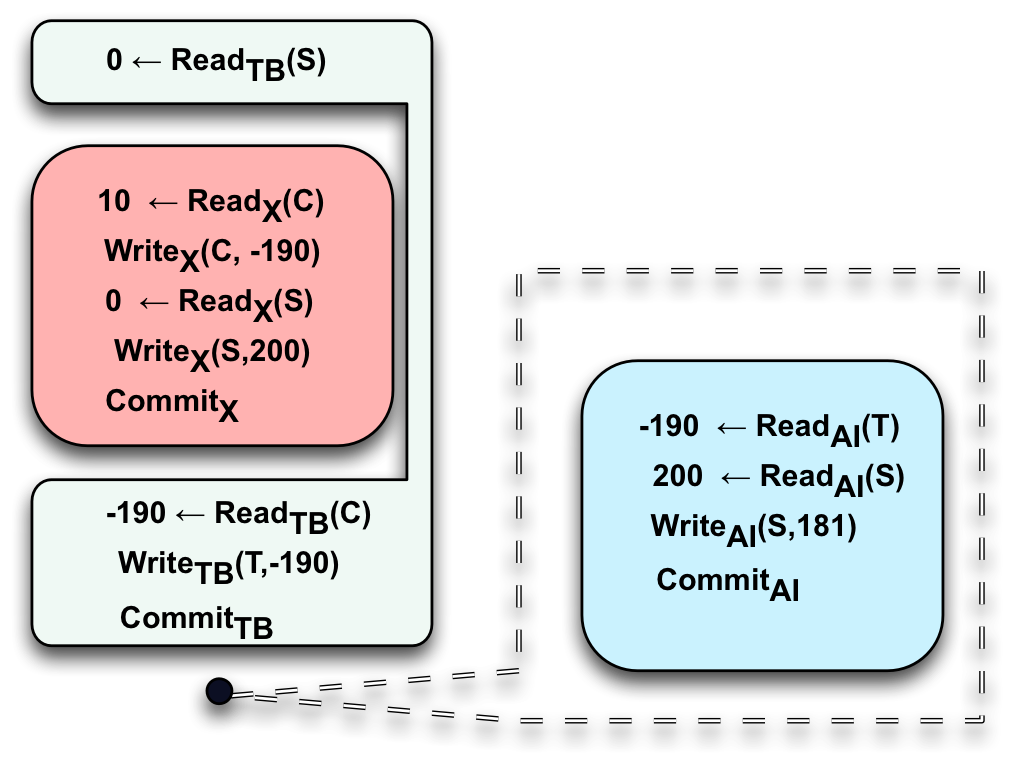
\includegraphics[scale=0.5]{Figures/motiv-eg-3-a}

\label{fig:motiv-eg-3-a}
\end{figure}

The subscripts X, TB and AI denote `Xfer', `TotBal' and `AddInt'
transactions, respectively. Assume that \C{C} and \C{S} are initially
10 and 0, respectively. Let \C{a} be 200, i.e., we subtract 200 from
\C{C} and add it to \C{S}.  This operation must be allowed because it
doesn't effect the total balance, hence the interest. The execution
begins with `TotBal' transaction reading the savings (\C{S}) balance
as 0 (we assume left-to-right evaluation order for \C{S + C}).
However, before it reads the current (\C{C}) balance, `Xfer'
transaction executes and commits, changing \C{C} to -190.
Subsequently, `TotBal' reads -190 from \C{C}, and updates \C{T} to
-190. `AddInt', which begins execution after `TotBal', reads -190 from
\C{T}, calculates interest as -19, and updates \C{S} to 181. The
result is a state with total balance as -190 + 181 = -9, thus
violating the invariant.

Note that transactions `Xfer' and `AddInt', which write to the data
objects (\C{C} and \C{S}) relevant to the invariant, are serialized in
the above execution. Transaction `TotBal' however is not. While
serializing it fixes the problem, it is not necessary. A simpler fix
is to isolate `TotBal' transaction from the effects of concurrent
`Xfer' transaction, so that it reads \C{C} as 10 despite the
concurrent `Xfer' transaction committing -190 to \C{C}. This can be
achieved by executing `TotBal' under \iso{Repeatable Read} (RR)
isolation level, which guarantees that any two reads of a data object
in a transaction return the same value (the \emph{repeatable reads}
property~\cite{berenson}). Allowing `Xfer' to interfere with `TotBal'
violates the repeatable read property since a hypothetical read from
\C{S} in `TotBal' after the interference returns a different value
(200) than the first read (0). Executing `TotBal' under RR restores
repeatable read by \emph{effectively} prohibiting such interference.

\begin{figure}[t]
\centering
\hspace*{-0.3in}$\{\{\texttt{V=0}\}\}$
\begin{tabular}{l||l}
\begin{txnimpcode}
  txn$\langle$'Rd'$\rangle${
    X := V
    Y := V
  }
\end{txnimpcode}
&
\begin{txnimpcode}
  cobegin (i $\leftarrow$ [1$\ldots$3]) {
    txn$\langle$'Inc['+i+']'$\rangle${
      V := V + 1
    }
  }
\end{txnimpcode}
% &
% \begin{txnimpcode}
%   txn$\langle$'Inc2'$\rangle${
%     V := V + 1
%   }
% \end{txnimpcode}
\\
\end{tabular}
\hspace*{-0.3in}$\{\{\texttt{Y}\ge\texttt{X}\}\}$

\caption{View counter (\C{V}) increments (\C{Inc}) and reads (\C{Rd})}
\label{fig:motiv-eg-4}
\end{figure}

Our last example demonstrates that it is not necessary to serialize
transactions, even those that write to the same data objects, to
maintain essential invariants in practical applications. Consider a
counter used to count video views on a YouTube-like application. The
counter need not accurately track the view count, but it must at least
ensure that the count does not decrease (nor does it appear to be
decreasing). Fig.~\ref{fig:motiv-eg-4} shows a simple example
involving a view counter (\C{V}). The three `Inc' transactions
(`Inc[1]' to `Inc[3]') increment the counter, while the transaction
`Rd' reads the counter twice and writes the values read to \C{X} and
\C{Y}, respectively. The count is 0 initially. Since we expect the
view count to monotonically increase, we require $\C{Y}\ge\C{X}$ at
the end. Under the standard setting, where new writes to data objects
always overwrite previous writes, the postcondition may not hold. For
instance, consider an execution where `Inc[1]' reads \C{V} as 0 (but
doesn't commit), then `Inc[2]' and `Inc[3]' commit serially changing
\C{V} to 2, followed by `Rd' reading 2 and writing it to \C{X}. Now
`Inc[1]', which has read \C{V} as 0 writes 1 to \C{V} and commits. The
subsequent read of \C{V} by `Rd' returns 1, which it writes to \C{Y}
and commits. In the final state, \C{X} is 2 and \C{Y} is 1, thus
violating the monotonicity invariant.

However, in an unconventional setting, such as a modern day replicated
data store, writes arriving at a replica need not necessarily
overwrite the existing writes. A \emph{conflict resolution strategy}
may be employed to pick, for example, a write with the largest value
among competing concurrent writes. Under this setting, the write to
\C{V} by `Inc[1]' with a value (1) less than the current value (2) is
discarded. Transaction `Rd' therefore continues to read 2, allowing it
to satisfy the postcondition. Note that we did not have to serialize
`Inc' transactions to uphold the monotonicity invariant, although they
are involved in Write-Write conflicts.  The default \iso{Read
Committed} isolation level suffices\footnote{We have implicitly assumed that
`Rd' transaction witnesses monotonically growing state, i.e., the
transactions that appear committed to the first read of \C{V} in `Rd'
also appear committed to the second read.  Most implementations of RC
enforce this \emph{Monotonic View} invariant. However,
some~\cite{pldi15,bailishat} categorize RC with Monotonic View as a
separate isolation level called \iso{Monotonic Atomic View} (MAV). On
those stores, we need MAV for `Rd'. }, provided that the conflict
resolution strategy consistently picks writes with larger values. A
reasoning framework for weak isolation must be sensitive to the
semantics of conflict resolution in order to formally prove the
monotonicity invariant in this example.

